\chapter{Discussion}
\label{c:discussion}
\IMRADlabel{discussion}



In this chapter we analyze the results from~\autoref{c:experiments} and set them into context with results from related work. We will split all the discussion on the different environments first and then discuss the overall performance of the \algname algorithm.

\section{Model Performance}
	\subsection{Proof-of-Concept: LGDS}
		As we have seen in~\autoref{fig:lgdsRollout}, the \ac{lgds} proof-of-concept environment works pretty well and the true data is perfectly predicted. Applying the \ac{nrmse} to the smoothed trajectory and the rollout, the model has an error of approximately \( 0.0001 \) for every metric. This shows that we are still able to learn linear dynamical systems. We expected this result as we have proven that our algorithm is equivalent to the \ac{lgds} inference algorithm for linear systems in~\autoref{app:ngkExactness}. Hence, our algorithm does not reduce the "power" of the linear algorithm on linear systems and only extends its usability to nonlinear systems.
	% end

	\subsection{Pendulum}
		\label{subsec:discussPendulum}

		The pendulum is the first environment where it gets really interesting as it is the first nonlinear environment we assess.

		As we have seen in the experiment for different latent dimensionalities, we need at least \(10\) latent dimensions to model the pendulum with a decent prediction error, where we expected some downsides on the prediction and expected a really good rollout in the training area. As we have seen in the results for a ten-dimensional latent in~\autoref{subsubsec:pendulumL10}, we see a good rollout in the training area and also a good prediction for the pendulum position, but a slightly smaller amplitude on the velocity side. This corresponds to an energy loss of the pendulum that should not happen as the pendulum is undamped.~\autoref{fig:pendulumEnergyL10} highlights this by showing the total, kinetic and potential energy of the system, where the rollout energy changes with time which should not happen. However, the potential energy almost matches the true potential energy, supporting our inspection that the position is well fit. The kinetic energy, generated by the velocity, is on the other hand a bit off. We can further inspect this behavior by looking at the rollout in the latent space in~\autoref{fig:pendulumLatentRolloutL10}. We see that the energy loss is primarily happening in the tenth dimension. Looking at the real parts of the eigenvalues of the latent state dynamics matrix,
		\begin{equation*}
			\sigma = \{ 1.00, 1.00, 1.00, 0.96, 0.65, 0.67, 0.86, 0.80, 0.73, 0.75 \}
		\end{equation*}
		we see that not all are close to one, \ie they vanish after some time. This directly corresponds to the energy loss in the system (the eigenvalues of a system capture the time evolution). We also see that the tenth dimension has a really high variance in its states, indicating that the model already has enough latent dimensions to explain the dynamics. Looking at the rollout of a nine-dimensional latent (run \texttt{58}) in~\autoref{fig:pendulumRolloutL09}, however, we see that the energy loss is still there. It does not make sense to inspect higher-dimensional latent spaces as we have seen in the latent dimensionalities experiment that the error does not shrink much. Additionally, the 14-dimensional latent that we inspected in~\autoref{subsubsec:pendulumL10} also looses energy. We do not expect this to get better with higher latent dimensionalities. Also, higher dimensionalities impose numerical instability, a phenomenon we will address in~\autoref{subsec:discussPerformanceNumerics}.

		For this environment, we get really small confidences with the true trajectory still lying in the region of confidence. We also see that the variance is higher on the turns of the pendulum which makes sense as that is the most critical part of the movement.

		While these first results cast a shadow on our model performance, the energy loss builds hope for the damped pendulum to work out well.

		\begin{figure}
			\centering
			\begin{subfigure}{0.7\linewidth}
				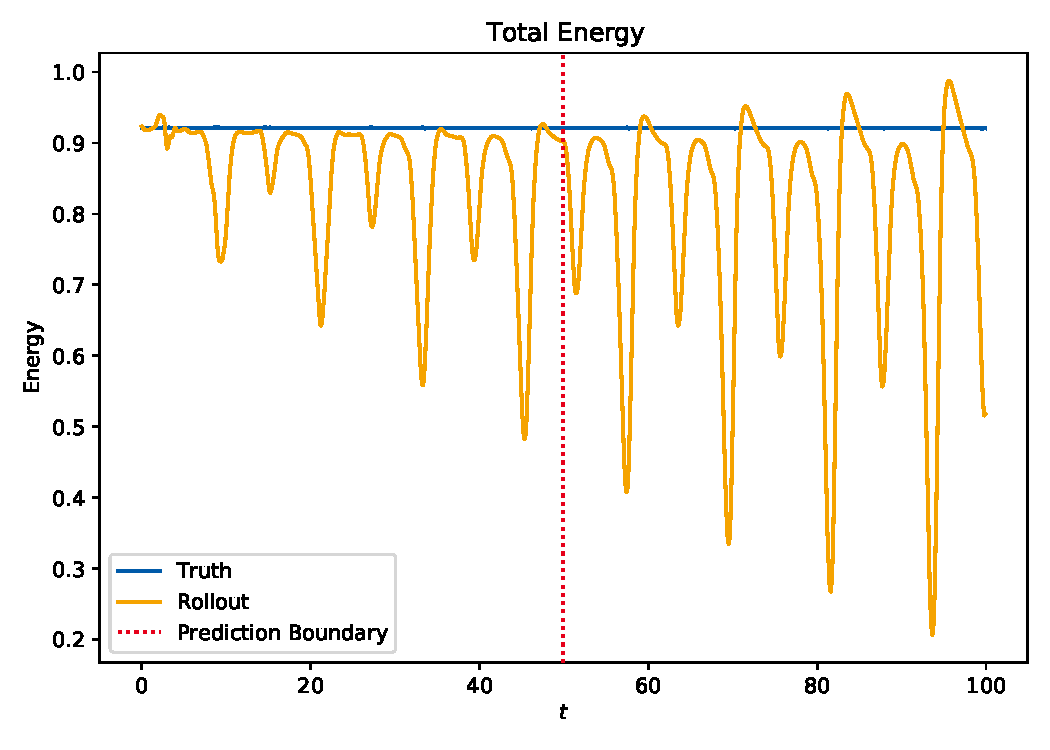
\includegraphics[width=\linewidth]{figures/results/pendulum/run-latent-dim-10/energy-R10-N0-total.png}
			\end{subfigure} \\
			\begin{subfigure}{0.5\linewidth}
				\centering
				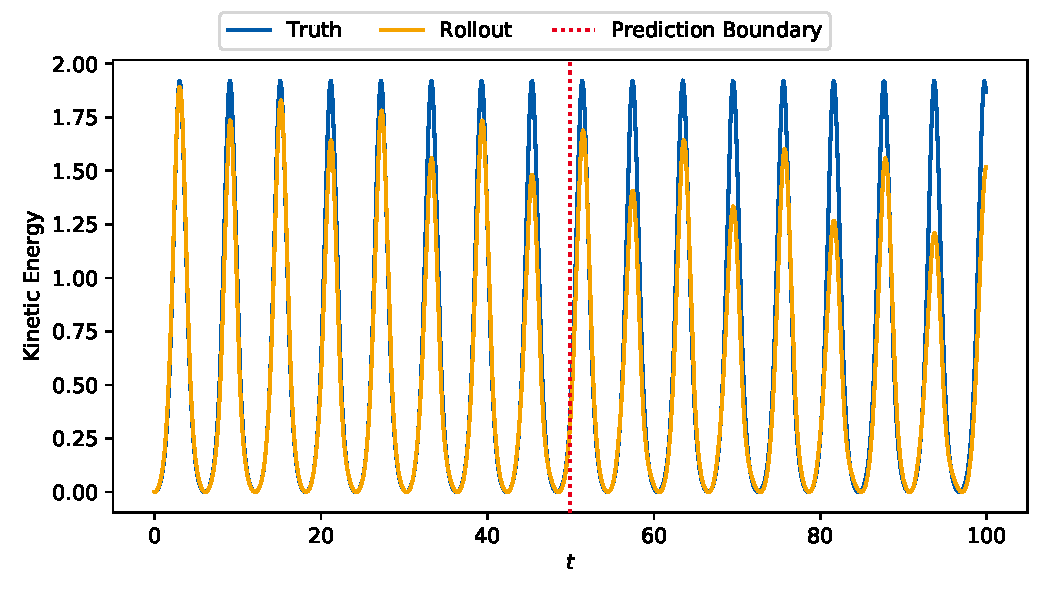
\includegraphics[width=\linewidth]{figures/results/pendulum/run-latent-dim-10/energy-R10-N0-kinetic.png}
			\end{subfigure}%
			~
			\begin{subfigure}{0.5\linewidth}
				\centering
				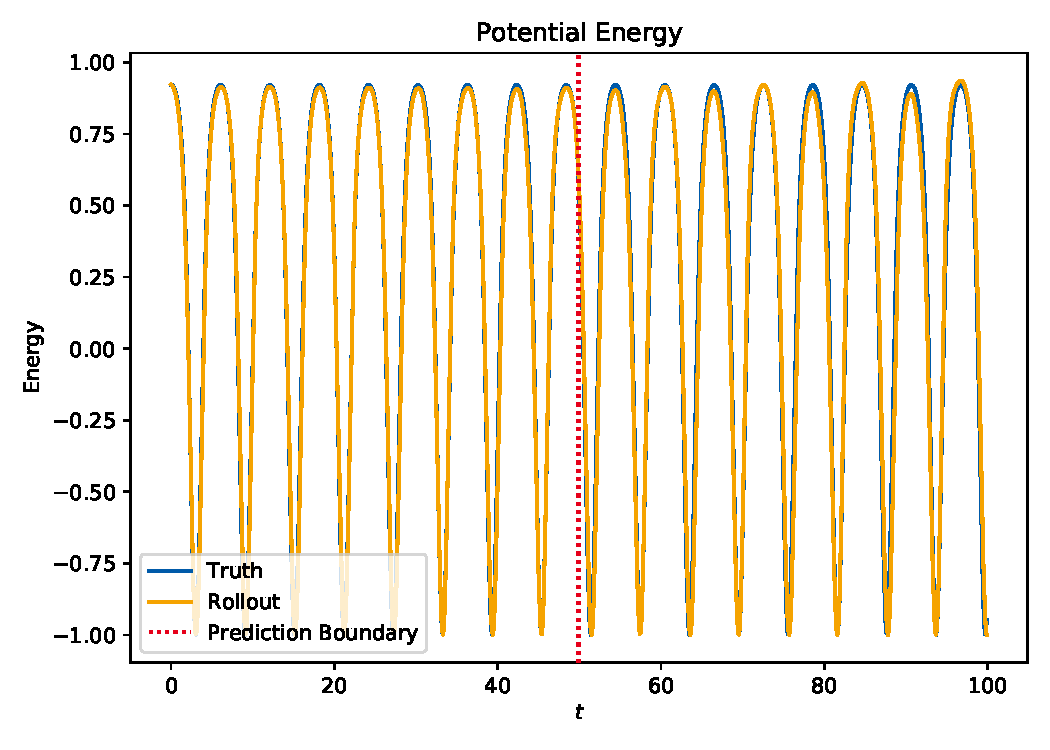
\includegraphics[width=\linewidth]{figures/results/pendulum/run-latent-dim-10/energy-R10-N0-potential.png}
			\end{subfigure}
			\caption[Total energy of the undamped pendulum]{Total energy of the undamped pendulum composed of the kinetic energy on the bottom left and the potential energy on the bottom right. The blue line represents the true energy, calculated from the training and validation data. The orange line is the energy calculated from the rollout. As usual, the red line is the prediction boundary until all training data was used and the rest is prediction.}
			\label{fig:pendulumEnergyL10}
		\end{figure}

		\begin{figure}
			\centering
			\includegraphics[width=\linewidth]{figures/results/pendulum/run-latent-dim-10/rollout-latents-N0.png}
			\caption[Latent rollout of the pendulum experiment for 10 latent dimensions]{Rollout of the latent dimensions of the pendulum environment for \(k = 10 \) latents.}
			\label{fig:pendulumLatentRolloutL10}
		\end{figure}

		\begin{figure}
			\centering
			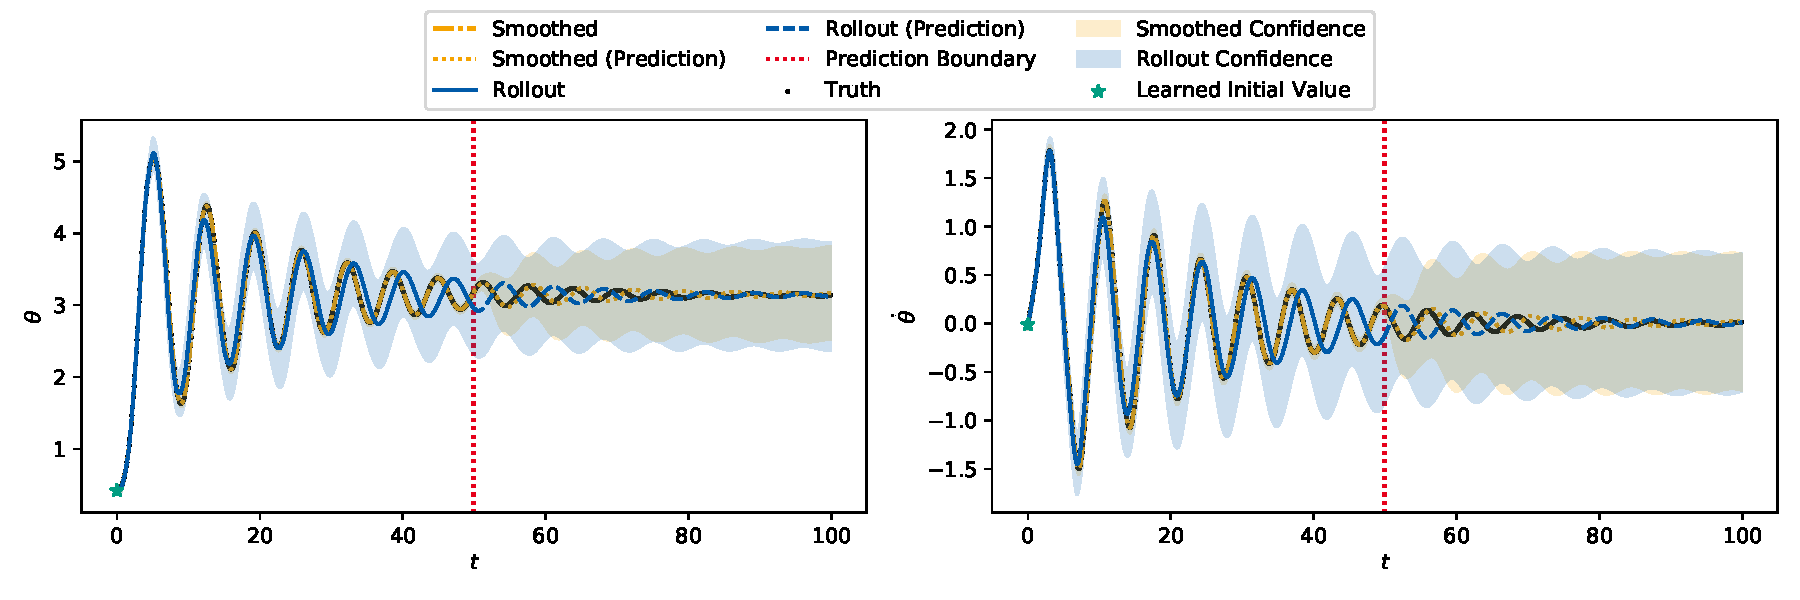
\includegraphics[width=\linewidth]{figures/results/pendulum/run-latent-dim-09/rollout-observations-N0.png}
			\caption[Rollout of the pendulum experiment for 9 latent dimensions]{The rollout plot in the observation space of the pendulum environment for \(k = 9\). The left plot shows the displacement and the right plot the angular velocity. The black dots represent the true data of which the model used everything till the red prediction boundary to train on. The blue line is the rollout, starting from the learned initial value (marked with a green star). The orange dash-dotted line is the smoothed data. The dotted orange line then is the rollout starting from the last smoothed state, forming the "smoothed prediction". The shaded regions show the confidence, \ie two times the standard deviation.}
			\label{fig:pendulumRolloutL09}
		\end{figure}
	% end

	\subsection{Damped Pendulum}
		\label{subsec:discussDampedPendulum}

		As for the undamped pendulum, we have seen in the experiment with different latent dimensionalities that we need at least ten latent dimensions. For ten dimensions, we get a decent \ac{nrmse} on both training and prediction. We have seen this behavior in~\autoref{subsubsec:pendulumDampedL10} and in the rollout plot in~\autoref{fig:pendulumDampedRolloutL10}. In contrast to the undamped pendulum, the amplitudes of the oscillations are now on the correct heights, so we definitely learn the energy loss of the system. We can also see this behavior in the plot of the total, kinetic and potential energy in~\autoref{fig:pendulumDampedEnergyL10}. We see in the total and the kinetic and potential energy that the damped pendulum model is really close to the real energy levels, in all energy types. This supports the first interpretation of the rollout that we really learn the energy loss. On the other hand, the rollout is phase-shifted to the real trajectory, sometimes even predicting the pendulum to be on the opposite side of a swing. Looking at the rollout in the latent space in~\autoref{fig:pendulumDampedLatentRolloutL10}, we see a similar behavior in the latent space, so our learned observation function seems to be correct, but the latent dynamics are a bit off.

		Improving this might be possible by fixing the observation function and optimizing just the state dynamics matrix on its own. This reduces the parameters the algorithm has to learn by a lot, possibly yielding a more accurate rollout. But overall we are satisfied with this result as we learn the energy loss and get a confidence that is not too high such that the real position is still in the region of variance. As for the undamped pendulum, we get higher variances in regions where the pendulum turns over.

		As the rollout is generated from a linear system in the background, it makes sense that energy-loosing systems can are easier to model: Taming a linear system to keep its energy for a long time is a lot harder than "letting it converge to zero". A stable non-zero system corresponds to eigenvalues that are approximately one (as \( \lim_{k \to \infty} 1^k = 1 \) and \( \lim_{k \to \infty} x^k = 0 \) for \( \lvert x \rvert < 1 \), but \( \lim_{k \to \infty} x^k \to \infty \) for \( x > 0 \)). Systems with eigenvalues close to one just have to be disturbed a little (\eg by inaccuracies) and the system diverges.

		\begin{figure}
			\centering
			\begin{subfigure}{0.7\linewidth}
				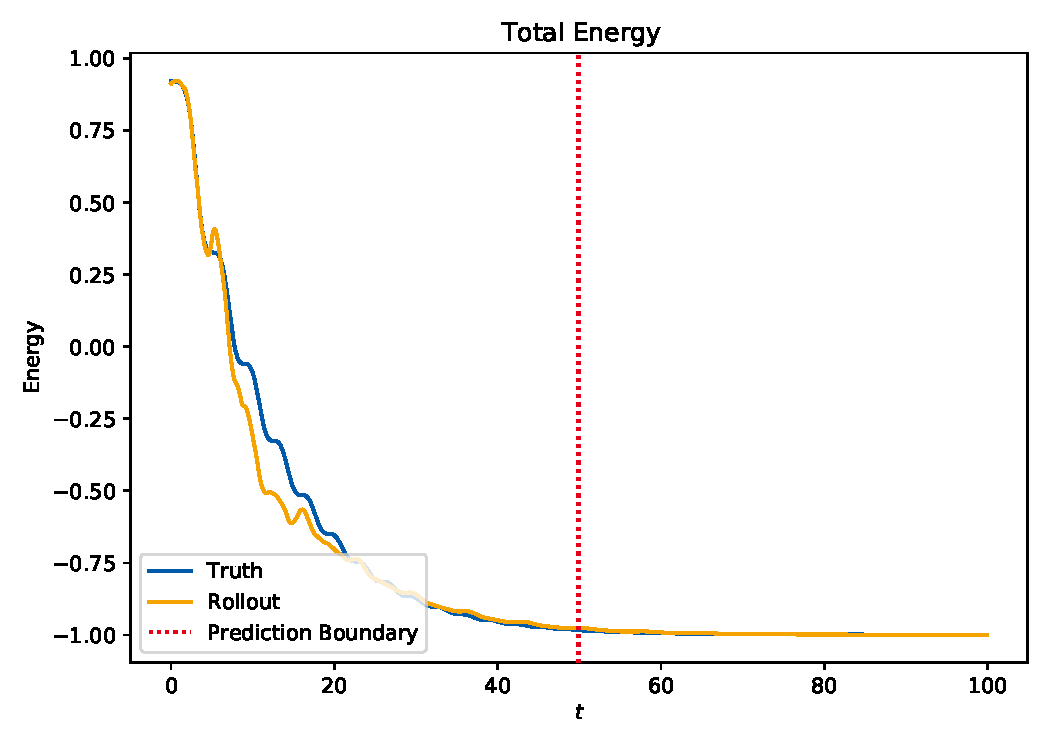
\includegraphics[width=\linewidth]{figures/results/pendulum-damped/run-latent-dim-10/energy-R110-N0-total.png}
			\end{subfigure} \\
			\begin{subfigure}{0.5\linewidth}
				\centering
				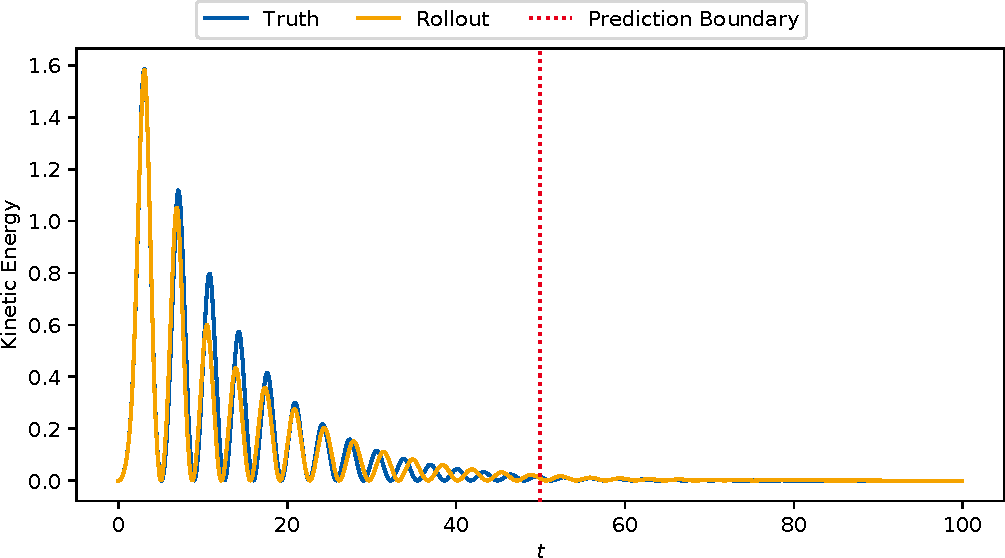
\includegraphics[width=\linewidth]{figures/results/pendulum-damped/run-latent-dim-10/energy-R110-N0-kinetic.png}
			\end{subfigure}%
			~
			\begin{subfigure}{0.5\linewidth}
				\centering
				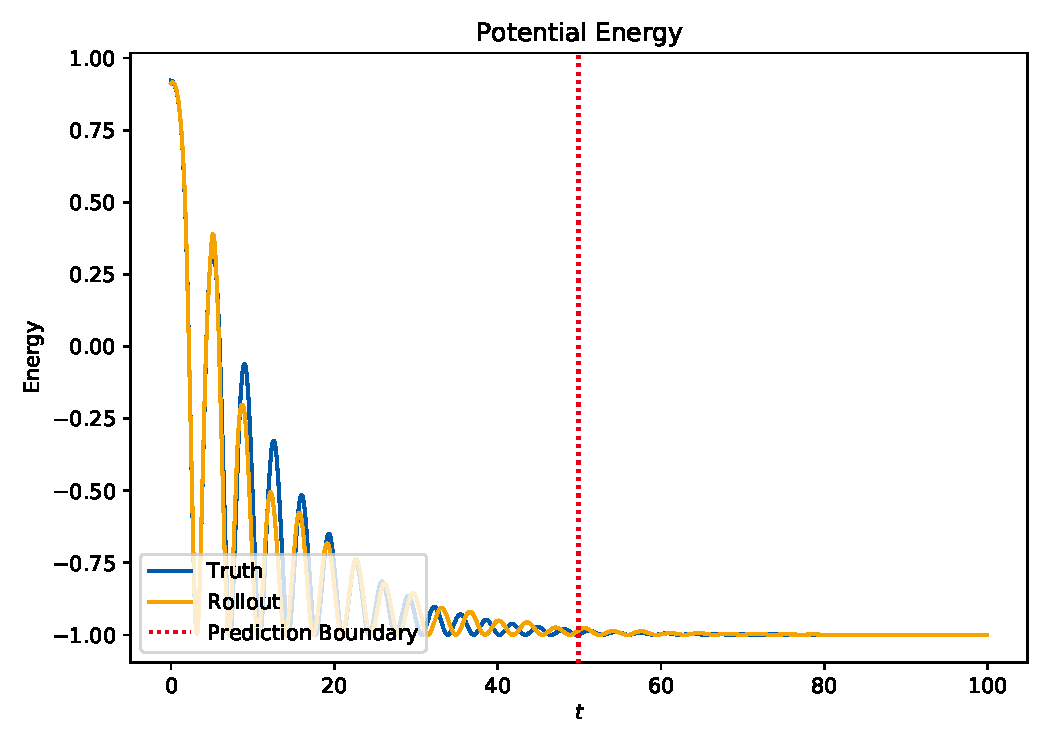
\includegraphics[width=\linewidth]{figures/results/pendulum-damped/run-latent-dim-10/energy-R110-N0-potential.png}
			\end{subfigure}
			\caption[Total energy of the damped pendulum]{Total energy of the damped pendulum composed of the kinetic energy on the bottom left and the potential energy on the bottom right. The blue line represents the true energy, calculated from the training and validation data. The orange line is the energy calculated from the rollout. As usual, the red line is the prediction boundary until all training data was used and the rest is prediction.}
			\label{fig:pendulumDampedEnergyL10}
		\end{figure}

		\begin{figure}
			\centering
			\includegraphics[width=\linewidth]{figures/results/pendulum-damped/run-latent-dim-10/rollout-latents-N0.png}
			\caption[Latent rollout of the damped pendulum experiment for 10 latent dimensions]{Rollout of the latent dimensions of the damped pendulum environment for \(k = 10 \) latents.}
			\label{fig:pendulumDampedLatentRolloutL10}
		\end{figure}
	% end

	\subsection{Gym Pendulum}
		\label{subsec:discussGymPendulum}

		As we have seen in the experiment with different latent dimensionalities in~\autoref{subsubsec:gymPendulumLatents}, we need at seven latent dimensions to get a decent \ac{nrmse} on the training rollout. However, we noticed that we get better results in one run for four latent dimensions (see~\autoref{subsubsec:gymPendulumL04}) which we looked at for a comparison with~\cite{mortonDeepVariationalKoopman2019a}. This shows that our algorithm is extremely sensitive on the initialization as the neural network is initialized randomly. Looking at the rollout of the seven-dimensional latent run in~\autoref{subsubsec:gymPendulumL07}, we see that the latent "stops to change" after the prediction boundary in comparison to the four-dimensional latent where the rollout still moves (and roughly captures the dynamics). By taking a look at the rollout in the latent space in~\autoref{fig:gymPendulumLatentRolloutL04} and~\autoref{fig:gymPendulumLatentRolloutL07} for the four- and seven-dimensional run, we see completely different time behaviors.

		As we have already outlined in~\autoref{subsec:discussDampedPendulum}, it is hard for a linear system to be stable when not converging to zero. We see such a behavior in the latent rollout: While the latents of the four-dimensional run all rise exponentially after the prediction horizon, causing movement in the observation space, approximately half of the latents in the seven-dimensional exponentially increase while the other half decreases exponentially. This seems to lead to vanishing withing the neural network, explaining the non-movement in the observation space. This behavior might be improved by regularizing the latent dynamics to a system with eigenvalues really close to one, leading to more stable dynamics. Another idea would be to make the latent dynamics time-dependent so compensate for the exploding states by adding an extra latent state just representing the time step. However, this would impose other difficulties and would make the system non-autonomous which is quite handy.

		Another interesting result of the Gym pendulum experiment is that it performs a lot worse than the simple angular pendulum in~\autoref{subsec:discussPendulum}. We have two possible reasons for this behavior: Firstly, the sine/cosine terms add more nonlinearity to the system (with small angle approximations it is possible to model the pendulum for small displacements, this is not possible using the sine/cosine of the angle). Secondly, taking the sine/cosine of the angle is actually a nonlinear feature transformation typically used to implicitly encode the symmetries in a polar coordinate environment like the pendulum. That is, the equality of \( 0 \triangleq 2\pi \) (swinging the pendulum around one time does not increase the angle by \(2\pi\), instead the pendulum works congruence class generalized to \(\R\)). Hence, we can also use the inverse feature transformation and recover the angle from the cosine/sine data and get similar performance as for the angular pendulum.

		\begin{figure}
			\centering
			\includegraphics[width=\linewidth]{figures/results/pendulum-gym/run-latent-dim-04/rollout-latents-N0.png}
			\caption[Latent rollout of the Gym pendulum experiment for 6 latent dimensions]{Rollout of the latent dimensions of the Gym pendulum environment for \( k = 6 \) latents.}
			\label{fig:gymPendulumLatentRolloutL04}
		\end{figure}
		\begin{figure}
			\centering
			\includegraphics[width=\linewidth]{figures/results/pendulum-gym/run-latent-dim-07/rollout-latents-N0.png}
			\caption[Latent rollout of the Gym pendulum experiment for 7 latent dimensions]{Rollout of the latent dimensions of the Gym pendulum environment for \( k = 7 \) latents.}
			\label{fig:gymPendulumLatentRolloutL07}
		\end{figure}
	% end

	\subsection{Gym Cartpole}
		As we have seen in the experiments with different latent dimensionalities in~\autoref{subsubsec:cartpoleLatents}, we need at least 10 latent dimensions to get a decent \ac{nrmse} on the (training) rollout. We have also seen that more latent dimensions (\eg 16 dimensions in~\autoref{subsubsec:cartpoleL16}) do not yield better results than ten latent dimensions (see~\autoref{subsubsec:cartpoleL10}). However, in both cases we get a near-to-perfect rollout before the prediction boundary but fail at the prediction. For the ten dimensional latent, the model captures the dynamics of the pole displacement/velocity and also the cart velocity after the prediction boundary roughly, but for the cart position the trajectory is quite off. Another interesting result is that the model is a lot more confident in the pole displacement and velocity than the cart position. Looking at just the data in~\autoref{fig:envCartpoleGym}, this makes sense. The movement of the car is more complex as it nonlinear acceleration only through the movement of the pendulum. This does not impose a linear movement on the cart, but rather it "wobbles" around zero\footnote{See \href{https://github.com/fdamken/bachelors-thesis/blob/b5a4acbc1d10fa0224a73201995222690d2fb6de/thesis/figures/cartpole.gif}{GitHub} for a GIF of the cartpole movement.}. Also, as we have seen in~\autoref{subsec:discussPendulum} and~\autoref{subsec:discussDampedPendulum}, we are able to learn the movement of an undamped and a damped pendulum, where the motion of the pole on a cart can be seen as a slightly damped pendulum as the system is transferring energy from the pendulum to the cart.

		\todo{Further improvements?}
	% end

	\subsection{Gym Double Pendulum}
		As we have seen in the experiment with different latent dimensionalities, we need at least 18 latent dimensions to model the double pendulum adequately in the training rollout. As expected from the \ac{nrmse}, we get a decent fit on the rollout for 18 latent dimensions (see~\autoref{fig:acrobotRolloutL18}), but the prediction is far off the true trajectory. The prediction does not even capture the dynamics roughly and also it is pretty certain on its wrong trajectory. This matches our expectations as the double pendulum is a chaotic environment with nonlinear coupling that is really hard to learn.

		Improving the performance on the double pendulum might be possible by using a shorter integration interval \(h\) to provide the algorithm more information between the states such that it can better extrapolate from the data. Another idea, similar to the one outlined in~\autoref{subsec:discussGymPendulum}, would be to apply an inverse feature transform on the sine/cosine of the angles to reduce the dimensionality of the observation space and let "the model discover the symmetries". We will discuss this again in~\nameref{sec:futureWork}. But overall we are satisfied that we managed to learn at least the rollout on the training data even in a chaotic system.
	% end

	\subsection{Running on the CPU or GPU Makes a Difference}
		\label{subsec:cpuGpu}

		We noticed that running our code on the \ac{cpu} or on the \ac{gpu} makes a huge difference in the quality of the results, where running on the \ac{gpu} is better. The environment we noticed the greatest difference is the double pendulum, of which we added two plots in~\autoref{app:plotsCpuGpu}.~\autoref{fig:cpuVsGpuCpu} shows the double pendulum experiment result running on the \ac{cpu} and~\autoref{fig:cpuVsGpuGpu} shows the double pendulum experiment result running on the \ac{gpu}. We expect both plots to be the same, but in fact the plot of the experiment running on the \ac{cpu} looks better. These runs are the runs \texttt{1564} and \texttt{1565}, respectively. In both cases we set the seed for both NumPy and PyTorch to the same value. As the data was generated beforehand, the Gym seed does not matter in this case. We expect this to be an issue with a gradient flowing too far through the computation graph or an issue with floating point operations working differently on the \ac{cpu}/\ac{gpu}.
	% end

	\subsection{Learning Multiple Sequences at Once}
		\label{subsec:singleMulti}

		We derived the Koopman inference algorithm in a way such that it should be possible to learn on multiple observation sequences at once (see~\autoref{sec:ngkDerivation}). However, we noticed that the results of learning from multiple sequences at once yields worse results than learning one observation sequence. We have multiple explanations for this issue, the most probable being an error in the implementation we did not find. Another explanation is that in the single-sequence case the neural network of the observation function overfits to the training data and does not have enough "memory" to also overfit to another observation sequence and therefore breaks. This is a serious problem to address and we might be able to overcome this problem by adding noise to the input to generalize better.

		\autoref{fig:plotsSingleSequence} and~\autoref{fig:plotsMultiSequence} show two rollouts on the damped pendulum environment, the former only learning on a single observation sequence and the latter learning on multiple sequences at once. We see that while the result of a single sequence captures the dynamics decently (see~\autoref{subsec:discussDampedPendulum} for an in-depth discussion), the model that learned on two sequences does not capture the dynamics correctly.
	% end

	\subsection{Discussion on Numerical Stability}
		\label{subsec:discussPerformanceNumerics}

		The primary thing we noticed in terms of numerical stability is the definiteness of the covariance matrices \(\mat{Q}\), \(\mat{R}\) and \(\mat{V}_0\). While this can be fixed by learning the Cholesky decomposition directly, better regularization or putting priors on the matrices (see~\autoref{sec:futureWork} for more information on these topics), we also faced singular matrices. This primarily happened for high latent dimensionalities, a phenomenon that can also be seen in the latent dimensionalities comparison plots in~\autoref{sec:results}. This is caused by the algorithm "not knowing what to do" with a latent dimension, \ie when it already has "enough" dimensions to explain the data. We could use this behavior to automatically detect which latents are important and which are not, called \emph{automatic relevance determination} (see~\autoref{subsec:ard}) for more proposals on this topic.

		With implementing the square-root filtering/smoothing in the E-step we gained a lot of numerical stability (also also speed) by not having to compute the Cholesky decomposition of every smoothed covariance.

		With all that combined, we are satisfied with the numerical stability of the Koopman inference algorithm, especially given that one of the great instabilities, singular matrices, lead to future work on automatic relevance determination.
	% end
% end

\section{Comparison with Related Work}
	% In-Depth Comparison with Lush et al.
	% In-Depth Comparsion with Morton et al.
	% Probably more qualitative comparisons with Sequential VAE or DVBF (Karl et al.).

	\todo{Exp: Comparison}
% end

%\section{Control}  % Only if there is time left!
%	% Introduce approach to control.
%	% Show results of LGDS control which is working.
%	% Highlight difficulties.
%
%	\todo{Discussion: Control}
%% end

\section{Future Work}
	\label{sec:futureWork}

	We will now discuss and propose future work and ideas that can be tried based on the results of this thesis.

	\subsection{Control}
		In this thesis we presented a method for learning a dynamical system with no control inputs. The most obvious extension would be to add control inputs to the latent space in an additive fashion \( \vec{s}_{t + 1} = \mat{A} \vec{s}_t + \mat{B} \vec{u}_t \) with a learnable control matrix \(\mat{B}\). With this approach it might be possible to actually perform \ac{mpc} and uncertainty-aware control like in~\cite{mortonDeepVariationalKoopman2019a}, but with a simpler model. Our first approach to this would be to test this method on a simple environment like the pendulum and first learn the control rollout and afterwards perform a stabilization task and try the swing-up of the pendulum.

		Looking into this was not possible for us as it is beyond the scope of this thesis.
	% end

	\subsection{Bayesian Treatment}
		Another extension would be to employ a Bayesian view on the parameters and treat \eg the state dynamics matrix, covariance matrices and so on as random variables. This would allow to gauge the uncertainty on the dynamics itself and would allow to restrict the matrices to small ones by placing a prior on them. The approach would be to remove the \ac{ml} estimator and marginalize over the parameters to get a predictive distribution. Another semi-Bayesian approach would be to use point-estimates using a \ac{map} estimator rather than a predictive distribution.
	% end

	\subsection{Automatic Relevance Determination (ARD)}
		\label{subsec:ard}

		In combination with going full Bayesian on the model goes the implementation of automatic relevance determination of latent dimensions as proposed in~\cite{bealVariationalKalmanSmoother2000} for linear systems. Choosing a zero-mean prior might lead to a determination of non-relevant latent states, driving the state dynamics matrix to zero. Implementing this could solve the problems described in~\autoref{subsec:discussPerformanceNumerics} that the algorithm does already have "enough" latent dimensions and drives the variance to a high level on some dimensions.
	% end

	\subsection{Better Regularization and Learning the Cholesky Decomposition}
		As already outlined in~\autoref{subsubsec:implRegularization}, it might be beneficial for numerical stability to directly learn the Cholesky decomposition of the covariance matrices by using numerical optimization instead of closed-form optimization. Another approach could be to impose better regularization on the matrices if they become negative (semi-) determinant. However, while giving this a short first try during our implementation, we found out that just adding some values to the diagonal does not lead to better model performance but rather drives the likelihood to negative infinity.

		As for control, we did not look further into this as we ran out of time and this is beyond the scope of this thesis. It should, however, not be too hard to implement.
	% end

	\subsection{Speed Improvements by Full PyTorch or Enhanced QR Decomposition}
		As the square-root smoothing heavily uses QR decompositions which are faster on the CPU but the M-step uses backpropagation which is faster on the GPU, we had to copy the data over in every \ac{em} iteration. It might be beneficial to implement a more advanced QR decomposition (\eg~\cite{andersonCommunicationAvoidingQRDecomposition2011a}) and run the whole algorithm in the GPU.
	% end

	\subsection{(Inverse) Feature Transformations}
		% TODO
	% end
% end
